\begin{figure}[htbp]
    \centering
    \subfloat[Top view.]{
        \begin{tikzpicture}[
            dimension/.style={draw, <->, >=stealth, thin, dashed, gray},
            pointer/.style={draw, ->, >=stealth, thin, gray}
        ]
            \node[anchor=south west, inner sep=0] (image) at (0,0) {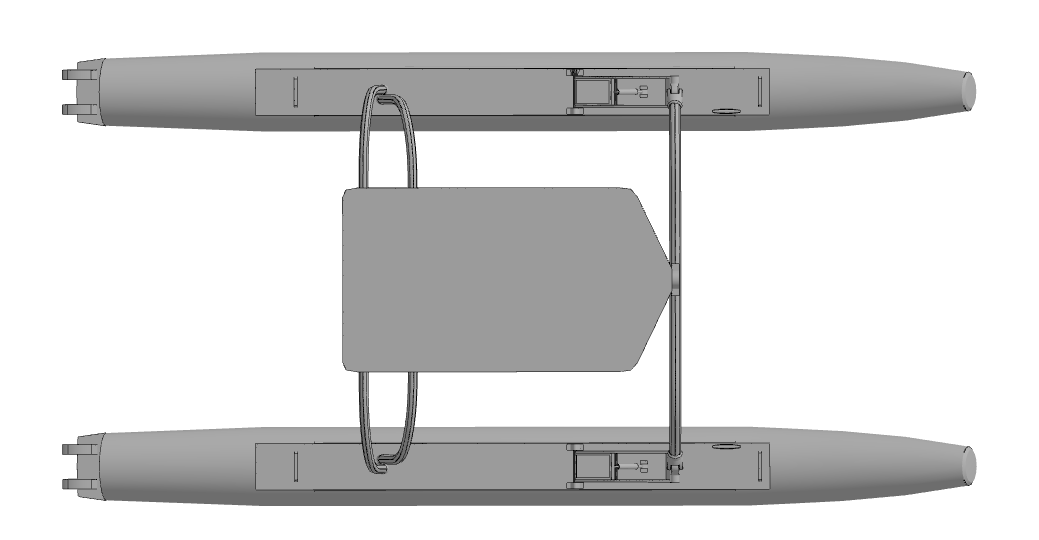
\includegraphics[width=0.40\textwidth]{Implementation/figures/01_simulation_environment/wamv_top_view.png}};
            \begin{scope}[x={(image.south east)},y={(image.north west)}]
                % Overall Length (4.90m)
                \draw[gray, thin] (0.06, 0.88) -- (0.06, 0.96);
                \draw[gray, thin] (0.94, 0.88) -- (0.94, 0.96);
                \draw[dimension] (0.06, 0.93) -- (0.94, 0.93);
                \node at (0.50, 0.96) [font=\tiny, above] {$4.90\,\text{m}$};

                % Overall Beam (2.40m nominal)
                \draw[gray, thin] (0.02, 0.07) -- (0.07, 0.07);
                \draw[gray, thin] (0.02, 0.92) -- (0.07, 0.92);
                \draw[dimension] (0.05, 0.07) -- (0.05, 0.92);
                \node at (0.05, 0.5) [font=\tiny, rotate=90, above] {$2.40\,\text{m}$};

                % Component Labels
                \node (hull_lbl) at (0.20, 0.50) [font=\tiny, draw, rounded corners=1pt, fill=white, inner sep=2pt] {Hulls};
                \draw[pointer] (hull_lbl.north) -- (0.30, 0.84);
                \draw[pointer] (hull_lbl.south) -- (0.30, 0.16);

                \node (deck_lbl) at (0.80, 0.35) [font=\tiny, draw, rounded corners=1pt, fill=white, inner sep=2pt] {Payload Deck};
                \draw[pointer] (deck_lbl.west) -- (0.55, 0.50);

                % Payload Deck Length (1.85m)
                \draw[gray, thin] (0.334, 0.3) -- (0.334, 0.23);
                \draw[gray, thin] (0.65, 0.3) -- (0.65, 0.23);
                \draw[dimension] (0.334, 0.27) -- (0.65, 0.27);
                \node at (0.50, 0.27) [font=\tiny, fill=white, inner sep=1pt] {$1.85\,\text{m}$};

                % Payload Deck Width (1.00m)
                \draw[gray, thin] (0.334, 0.315) -- (0.29, 0.315);
                \draw[gray, thin] (0.334, 0.65) -- (0.29, 0.65);
                \draw[dimension] (0.31, 0.315) -- (0.31, 0.65);
                \node at (0.31, 0.495) [font=\tiny, rotate=90, fill=white, inner sep=1pt] {$1.00\,\text{m}$};
            \end{scope}
        \end{tikzpicture}
        \label{fig:wamv_top}
    }
    \hfill
    \subfloat[Side view.]{
        \begin{tikzpicture}[
            dimension/.style={draw, <->, >=stealth, thin, dashed, gray}
        ]
            \node[anchor=south west, inner sep=0] (image) at (0,0) {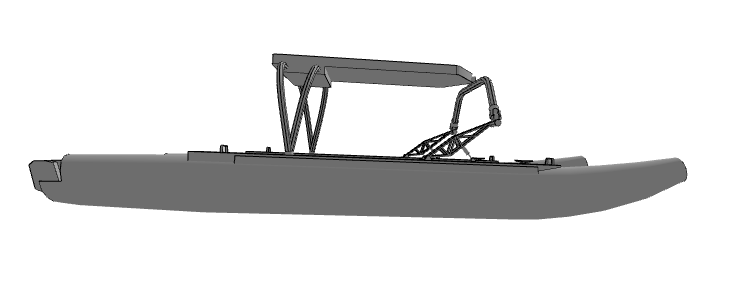
\includegraphics[width=0.40\textwidth]{Implementation/figures/01_simulation_environment/wamv_side_view.png}};
            \begin{scope}[x={(image.south east)},y={(image.north west)}]
                % Water Level
                \draw[gray, thick, dashed] (0.02, 0.28) -- (0.92, 0.28) node[right, font=\tiny] {Water Level};

                % Deck Height (1.25m above water level)
                \draw[gray, thin] (0.64, 0.77) -- (0.75, 0.77);
                \draw[gray, thin] (0.68, 0.28) -- (0.75, 0.28);
                \draw[dimension] (0.72, 0.28) -- (0.72, 0.77);
                \node at (0.72, 0.525) [font=\tiny, right] {$1.25\,\text{m}$};
            \end{scope}
        \end{tikzpicture}
        \label{fig:wamv_side}
    }
    \caption{WAM-V catamaran layout.}
    \label{fig:wamv_schematic}
\end{figure}